\documentclass{VUMIFPSkursinis}
\usepackage{algorithmicx}
\usepackage{algorithm}
\usepackage{algpseudocode}
\usepackage{amsfonts}
\usepackage{amsmath}
\usepackage{bm}
\usepackage{caption}
\usepackage{paralist}
\usepackage{color}
\usepackage{float}
\usepackage{graphicx}
\usepackage{listings}
\usepackage{subfig}
\usepackage{wrapfig}
\usepackage{enumitem}% http://ctan.org/pkg/enumitem

% Titulinio aprašas
\university{Vilniaus universitetas}
\faculty{Matematikos ir informatikos fakultetas}
\department{Programų sistemų katedra}
\papertype{Kursinis darbas}
\title{Gestų kalbos atpažinimas naudojant įprastą web kamerą}
\titleineng{Sign language recognition using web camera}
\status{3 kurso I grupės studentas}
\author{Pranciškus Ambrazas}
\supervisor{asist. Linas Petkevičius}
\date{Vilnius, \the\year}

% Nustatymai
% \setmainfont{Times New Roman}   % Pakeisti teksto šriftą į Palemonas (turi būti įdiegtas sistemoje)
\bibliography{bibliografija}

\begin{document}
\maketitle

\tableofcontents

\sectionnonum{Įvadas}
Pasaulyje šiuo metu apie 70 milijonų kurčių žmonių (https://wfdeaf.org/faq/). Šie žmonės dažniausiai komunikuoja su kitais gestų kalba, kai kurie net moka skaityti iš lūpų. Kiekviena pasaulyje esanti kalba turi ir savo gestų kalbą.Tai reiškia, skiriasi tiek gestų kalbos gramatika, tiek netgi patys gestai. Pasaulyje randama net dialektų pagal regionus, ne tik pagal šalis. Pavyzdžiui, amerikiečių anglų kalba šnekančių žmonių pasaulyje yra apie 500 tūkstančių (remiantis United States Census Bureau’s data from the 2009-2013 American Community Survey). Todėl bendraujant dviem žmonėm, mokantiems gestų kalbą neretai iškyla vertimų problema, todėl tenka ieškoti gestų vertimų. Paiešką galima atlikti atsižvelgiant į delno padėtį, rankos judesį (ar net abiejų rankų), rankos padėtį ir kiek rankų atlieka gestą. Tuomet pagal gesto išvaizdos paveiksliukus ar kartais net vaizdo įrašus, gestakalbiai gali išsiversti gestus.Tam yra skirtos tiek internetinės svetainės - žodynai, tiek įvairūs rašytiniai žodynai.


Gestų kalba ir jos atpažinimas yra viena iš daugelio apsimokančių sistemų sričių ir jau daug atlikta darbo nagrinėjant šią temą.
Yra daug įvairių pavyzdžių, kaip sistemos atpažįsta gestų kalbos abėcėlę ar net sugeba pačios perskaityti žodžius, apjungti juos į sakinius, o kai kurios net ir atsakyti naudojant gestų kalbą.
Pati gestų kalba susideda iš dviejų dalių: abėcėlės, kuri atvaizduojama statiniais judesiais, ir žodžių ar jų junginių, kurie atvaizduojami dinaminiais judesiais.

Pagrindinės problemos iškylančios atpažįstant statinius gestų kalbos ženklus yra:
\setdefaultleftmargin{2cm}{}{}{}{}{}
\setlist[enumerate]{noitemsep, topsep=0pt}
\begin{enumerate}
	\item Kiekvienos kalbos abėcėlę sudaro skirtingas raidžių (statinių ženklų) skaičius. \textit{Pavyzdžiui}, lietuvių kalbos abėcėlę sudaro 32 ženklai, o amerikietišką - 26; 
	\item Gestų panašumai. \textit{Pavyzdžiui}, raidės A, E, N, S, T yra atvaizduojamos sugniaužtus kumštį, o net trijose iš jų (A, E ir S) skiriasi tik nykščio padėtis;
	\item Kampas, kuris susidaro atpažįstant gestą. \textit{Pavyzdžiui}, kai A raidė rodoma ne iš priekio, o iš šono;
	\item Apšvietimas. \textit{Pavyzdžiui}, gestų atpažinimas esant prieblandai ir dienos šviesai.
\end{enumerate}

Pagrindinės problemos iškylančios atpažįstant dinaminius gestų kalbos ženklys yra:
\begin{enumerate}
	\item Nauji gestų kalbos žodžiai. \textit{Pavyzdžiui}, kiekvienas uraganas turi savo pavadinimą, todėl tai gali reikšti naujo gesto atsiradimą; 
	\item Gesto kelios reikšmės. \textit{Pavyzdžiui}, vienas gestas gali turėti kelias reikšmes, kaip kad lietuvių kalboje vienas žodis „kasa“ gali turėti net tris skirtingas reikšmes;
	\item Kampas, kuris susidaro atpažįstant gestą. \textit{Pavyzdžiui}, kai A raidė rodoma ne iš priekio, o iš šono;
	\item Žodžių apjungimas į vieną sakinį. \textit{Pavyzdžiui}, keli gestai einantys vienas po kito gali reikšti vieną žodį, tačiau tuo pačiu būti panašūs į vieną gestą, kuris jau reikš tik vieną žodį.
\end{enumerate}

Įvade apibūdinamas darbo tikslas, temos aktualumas ir siekiami rezultatai.
Darbo įvadas neturi būti dėstymo santrauka. Įvado apimtis 1–2 puslapiai.

\section{Medžiagos darbo tema dėstymo skyriai}
Medžiagos darbo tema dėstymo skyriuose pateikiamos nagrinėjamos temos detalės:
pradinė medžiaga, jos analizės ir apdorojimo metodai, sprendimų įgyvendinimas,
gautų rezultatų apibendrinimas. Šios dalies turinys labai priklauso nuo darbo
temos. Skyriai gali turėti poskyrius ir smulkesnes sudėtines dalis, kaip
punktus ir papunkčius.

Medžiaga turi būti dėstoma aiškiai, pateikiant argumentus. Tekstas dėstomas
trečiuoju asmeniu, t.y. rašoma ne „aš manau“, bet „autorius mano“, „autoriaus
nuomone“. Reikėtų vengti informacijos nesuteikiančių frazių, pvz., „...kaip jau
buvo minėta...“, „...kaip visiems žinoma...“ ir pan., vengti grožinės literatūros
ar publicistinio stiliaus, gausių metaforų ar panašių meninės išraiškos
priemonių.

\subsection{Poskyris}
Citavimo pavyzdžiai: cituojamas vienas šaltinis \cite{PvzStraipsnLt}; cituojami
keli šaltiniai \cite{PvzStraipsnEn, PvzKonfLt, PvzKonfEn, PvzKnygLt, PvzKnygEn,
PvzElPubLt, PvzElPubEn, PvzMagistrLt, PvzPhdEn}.

\subsubsection{Skirsnis}
\subsubsubsection{Straipsnis}
\subsubsection{Skirsnis}
\section{Skyrius}
\subsection{Poskyris}
\subsection{Poskyris}

\sectionnonum{Rezultatai ir išvados}
Rezultatų ir išvadų dalyje turi būti aiškiai išdėstomi pagrindiniai darbo
rezultatai (kažkas išanalizuota, kažkas sukurta, kažkas įdiegta) ir pateikiamos
išvados (daromi nagrinėtų problemų sprendimo metodų palyginimai, teikiamos
rekomendacijos, akcentuojamos naujovės).

\printbibliography[heading=bibintoc]  % Šaltinių sąraše nurodoma panaudota
% literatūra, kitokie šaltiniai. Abėcėlės tvarka išdėstomi darbe panaudotų
% (cituotų, perfrazuotų ar bent paminėtų) mokslo leidinių, kitokių publikacijų
% bibliografiniai aprašai.  Šaltinių sąrašas spausdinamas iš naujo puslapio.
% Aprašai pateikiami netransliteruoti. Šaltinių sąraše negali būti tokių
% šaltinių, kurie nebuvo paminėti tekste.

% \sectionnonum{Sąvokų apibrėžimai}
\sectionnonum{Santrumpos}
Sąvokų apibrėžimai ir santrumpų sąrašas sudaromas tada, kai darbo tekste
vartojami specialūs paaiškinimo reikalaujantys terminai ir rečiau sutinkamos
santrumpos.

\appendix  % Priedai
% Prieduose gali būti pateikiama pagalbinė, ypač darbo autoriaus savarankiškai
% parengta, medžiaga. Savarankiški priedai gali būti pateikiami ir
% kompaktiniame diske. Priedai taip pat numeruojami ir vadinami. Darbo tekstas
% su priedais susiejamas nuorodomis.

\section{Niauroninio tinklo struktūra}
\begin{figure}[H]
    \centering
    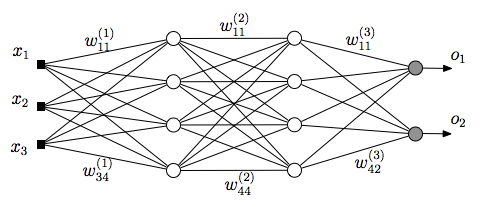
\includegraphics[scale=0.5]{img/MLP}
    \caption{Paveikslėlio pavyzdys}
    \label{img:mlp}
\end{figure}


\section{Eksperimentinio palyginimo rezultatai}
% tablesgenerator.com - converts calculators (e.g. excel) tables to LaTeX
\begin{table}[H]\footnotesize
  \centering
  \caption{Lentelės pavyzdys}
  {\begin{tabular}{|l|c|c|} \hline
    Algoritmas & $\bar{x}$ & $\sigma^{2}$ \\
    \hline
    Algoritmas A  & 1.6335    & 0.5584       \\
    Algoritmas B  & 1.7395    & 0.5647       \\
    \hline
  \end{tabular}}
  \label{tab:table example}
\end{table}

\end{document}
